%%%%%%%%%%%%%%%%%%%%%%%%%%%%%%%%%%%%%%%%%%%%%%%%%%%%%%%%%%%%%%%%%%%%%%%%%%%%%%%%
%2345678901234567890123456789012345678901234567890123456789012345678901234567890
%1         2         3         4         5         6         7         8
 
% to do:
% 1, change the article according to Shen
% 2, change according to the tutor
% 3, open source
 
\documentclass[letterpaper, 10 pt, conference]{ieeeconf}  % Comment this line out if you need a4paper
 
%\documentclass[a4paper, 10pt, conference]{ieeeconf}      % Use this line for a4 paper
 
\IEEEoverridecommandlockouts                              % This command is only needed if 
                                                         
% you want to use the \thanks command
 
\overrideIEEEmargins                                      % Needed to meet printer requirements.
 
% See the \addtolength command later in the file to balance the column lengths
% on the last page of the document
 
% The following packages can be found on http:\\www.ctan.org
%\usepackage{graphics} % for pdf, bitmapped graphics files
%\usepackage{epsfig} % for postscript graphics files
%\usepackage{mathptmx} % assumes new font selection scheme installed
%\usepackage{times} % assumes new font selection scheme installed
%\usepackage{amsmath} % assumes amsmath package installed
%\usepackage{amssymb}  % assumes amsmath package installed
 
\usepackage{url}
\usepackage{cite}
\usepackage{times}
%\usepackage{epsfig}
\usepackage{graphicx}
\usepackage{amsmath}
\usepackage{amssymb}
\usepackage{enumerate}
\usepackage{mathtools}
\usepackage{amsmath}
\usepackage{algorithm}  
\usepackage{algorithmic}
\DeclareMathOperator*{\argmax}{argmax}
\DeclareMathOperator*{\argmin}{argmin}
\usepackage{subfigure}
\usepackage{float}
%\usepackage{caption}
\usepackage{multirow}
% \usepackage{flushend}
  
\title{\LARGE \bf
Flow-Motion and Depth Network for Monocular Stereo and Beyond
\\ --Supplementary Material--
}
 
\author{Kaixuan Wang and Shaojie Shen
\\
\\ \url{https://github.com/HKUST-Aerial-Robotics/Flow-Motion-Depth}% <-this % stops a space
\thanks{All authors are with the Department of ECE, HKUST, Hong Kong, China. {\tt\small \{kwangap, eeshaojie\}@ust.hk}}
}
 
%\thanks{*This work was not supported by any organization}% <-this % stops a space
%\thanks{$^{1}$Albert Author is with Faculty of Electrical Engineering, Mathematics and Computer Science, University of Twente, 7500 AE Enschede, The Netherlands {\tt\small albert.author@papercept.net}}%
%\thanks{$^{2}$Bernard D. Researchers with the Department of Electrical Engineering, Wright State University, Dayton, OH 45435, USA {\tt\small b.d.researcher@ieee.org}}%
 
%\resetconfstandarts
%--------------------------------------------------------------------------
 
\begin{document}
 
%%%%%%%%% TITLE
% \title{Flow-Motion and Depth Network for Multiview Structure-from-Motion
% \\-- Supplementary Material --}
 
% \author{Kaixuan Wang, Shaojie Shen\\
% Hong Kong University of Science and Technology\\
% Hong Kong\\
% {\tt\small kwangap@ust.hk, eeshaojie@ust.hk}
% % For a paper whose authors are all at the same institution,
% % omit the following lines up until the closing ``}''.
% % Additional authors and addresses can be added with ``\and'',
% % just like the second author.
% % To save space, use either the email address or home page, not both
% % \and
% % Second Author\\
% % Institution2\\
% % First line of institution2 address\\
% % {\tt\small secondauthor@i2.org}
% }
 
% \title{\LARGE \bf
% Flow-Motion and Depth Network for Monocular Stereo and Beyond
% \\-- Supplementary Material --
% }
 
% \author{Kaixuan Wang, Shaojie Shen\\
% Hong Kong University of Science and Technology\\
% Hong Kong\\
% {\tt\small kwangap@ust.hk, eeshaojie@ust.hk}
 
\maketitle
%\thispagestyle{empty}
 
\begin{abstract}
   
This supplementary material provides more details about the proposed method, training, and dataset. More qualitative results of the experiments are provided as a supplement to the main letter. To demonstrate the generalization ability of the network and the effectiveness of the GTA-SfM dataset, the trained network is also directly applied to unseen scenes. Finally, we discuss the advantages and limitations of the proposed method.
\end{abstract}
 
%%%%%%%%% BODY TEXT
\section{Network Details}
 
In this section, we introduce more details in the flow-motion network and depth network. The depth observability of the epipolar point is also discussed in this section.
 
\subsection{Flow Regularization}
 
With an estimated optical flow $\mathbf{w}$, a regularized flow $\mathbf{w}_r$, is calculated such at the corresponding pixels are constrained on epipolar lines. For each pixel $\mathbf{x}_s$ on the source image, the regularized flow $\mathbf{w}_r(\mathbf{x}_s)$ is calculated by
\begin{equation}
    \scalebox{0.95}{$
    \begin{aligned}
    &\mathop{\arg\min}_{\mathbf{w}_r(\mathbf{x}_s)} && \lVert \mathbf{w}_r(\mathbf{x}_s) - 
    \mathbf{w}(\mathbf{x}_s) \rVert_2 \\
    &\text{subject to} && \begin{bmatrix} \mathbf{x}_s + \mathbf{w}_r(\mathbf{x}_s) \\ 1 \end{bmatrix}^T F \begin{bmatrix} \mathbf{x}_s \\ 1 \end{bmatrix} = 0
    \end{aligned}$}.
\end{equation}
$\mathbf{w}_r(\mathbf{x}_s)$ can be solved as Equation 3 in the main letter.
 
\subsection{Pixel Search Space}
 
$F [\mathbf{x}_s, 1]^T$ is the epipolar line on the target image. For notational simplicity, let $[e_x, e_y, e_z]^T = $ $F [\mathbf{x}_s, 1]^T$. $\mathbf{h} = [e_y, -e_x] / (e_x^2+e_y^2)$ is the normalized vector of the epipolar line direction. One the contrary, $\mathbf{v} = [e_x, e_y] / (e_x^2+e_y^2)$ is the vector perpendicular to $\mathbf{h}$. With $\mathbf{h}$ and $\mathbf{v}$, we define the search space in the target feature map $\mathbf{f}_t$ as Equation 4 in the main letter.
 
\subsection{Depth Observability}
 
The epipolar point in the source image is \scalebox{0.85}{$\mathbf{x}_e = \lambda(-KR^{-1}\mathbf{t})$}. For any pixel depth $d$, the point is projected onto the target image as the same point,
\begin{equation}
\begin{aligned}
\mathbf{x}_t & = \lambda(KRK^{-1}[\mathbf{x}_e, 1]^T \cdot d + K\mathbf{t}) \\
                 & = \lambda(KRK^{-1}[\lambda(-KR^{-1}\mathbf{t}), 1]^T \cdot d + K\mathbf{t}) \\
                 & = \lambda(K\mathbf{t})
\end{aligned},
\end{equation}
thus the depth $d$ is unobservable.
 
For the stereo configuration, $\mathbf{x}_e$ is at infinity so that all pixels in the image can be triangulated. However, in some unconstrained SfM cases, the epipolar point is on the image and cannot be triangulated directly. DeMoN~\cite{demon} uses networks to refine triangulated depth maps with NaN values set to 0. Li \textit{et. al.}~\cite{freeze_people} set pixels around the camera epipolar to zero. We believe the proposed triangulation layer is an alternative solution.
 
% \subsection{Network Definition} 
 
% The detailed definition of the networks used in multiview estimation is provided in Table~\ref{fig:architecture_table} and Table~\ref{fig:architecture_table2}. Two-view depth estimation (Figure 5(a) in the main paper) is a simple encoder-decoder network similar to Table~\ref{fig:architecture_table2}(b).
 
% \section{Dataset}
 
% The MVS-Synth
 
\section{Training}
 
Since the proposed method decouples the two-view SfM problem into flow-motion estimation and depth triangulation, we train the two networks separately. The flow-motion network is first trained and then is used to train the depth network with weight fixed. Adam optimizer~\cite{adam} is used and the initial learning rate is set to 1e-4. We half the learning rate when the error plateaus. Only color augmentation is used in the training.
 
\section{GTA-SfM dataset}
 
In this letter, we propose a GTA-SfM dataset which is used for the network training. A similar dataset, MVS-Synth, is also rendered in GTA5 environment. In MVS-Synth, cameras usually move randomly with small translations. On the contrary, in the proposed dataset, the trajectory is manually defined that cameras move in large translations and rotations.
 
We provide samples of the dataset in Figure~\ref{fig:dataset_compare}. As shown in the figure, the proposed dataset is more similar to that of SfM applications.
 
\begin{figure*}[h]
\vspace{0.5cm}
\begin{center}
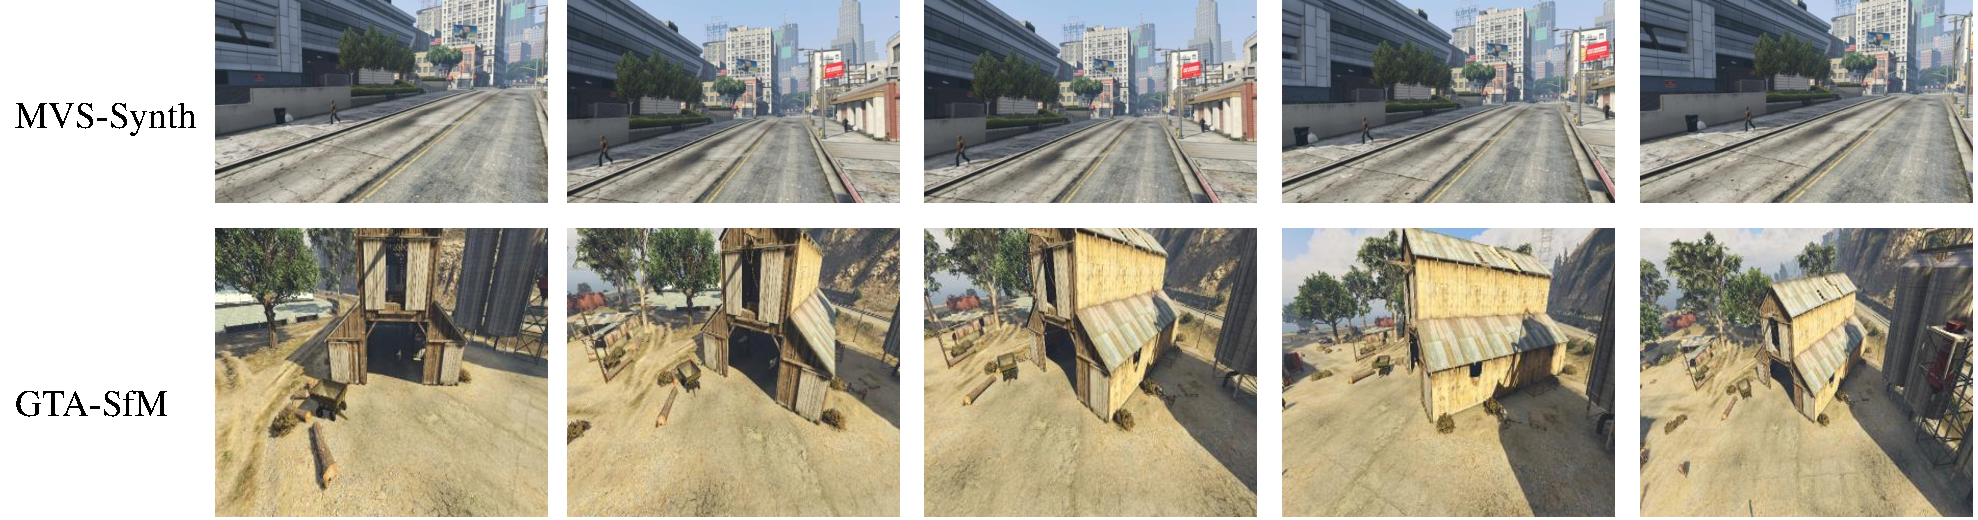
\includegraphics[width=1.0\linewidth]{figs/dataset_compare.pdf}
\end{center}
\vspace{-0.5cm}
\caption{Compare the proposed GTA-SfM dataset and previous MVS-Synth dataset. The trajectory of the camera in the proposed dataset contains large translation and rotation.}
\label{fig:dataset_compare}
\end{figure*}
 
\section{Experiments}
 
\subsection{Two-view Evaluation}
 
\textbf{Pose Estimation} Camera poses are estimated using optical flow in different resolutions. Here, we study the pose estimation quality together with the corresponding optical flow quality. The result is shown in Table~\ref{multi_pose}. At finer pyramid levels, the error of both optical flow and camera pose estimation decreases. However, contrary to the experience from classic SfM methods, the camera pose estimation is still better than SIFT even the optical flow resolution is $40\times32$. This can be explained by the dense pixel correspondences from the optical flow. 
 
\begin{table}[h]
\centering
\caption{Camera pose and optical flow estimation quality at different pyramid levels.}
\label{multi_pose}
\scalebox{0.95}{
\begin{tabular}{c|cccc}
Level & Resolution & Flow Err. & Rot. Err. & Trans. Err. \\ \hline
0     & 160$\times$128    & 3.168      & 1.491      & 8.517        \\
1     & 80$\times$64      & 3.269      & 1.566      & 8.559        \\
2     & 40$\times$32      & 3.707      & 1.776      & 10.630       \\ \hline
\end{tabular}}
    % \vspace{0.1cm}
    % \vspace{-0.3cm}
\end{table}
 
\textbf{Depth Estimation} As shown in Figure~\ref{fig:sup_demon}, we provide more qualitative results of our method on the DeMoN dataset. In MVS sequence, the depth net has difficult estimating the structure of trees such as the second, and the fourth row. These trees usually have very complex structures and introduce occlusions. Such structures and are difficult even for offline methods (the ground truth also misses the trees).
 
\subsection{Depth Fusion Evaluation}
 
\textbf{Qualitative Results} Multiview images bring more structure information of the scene, thus the depth map estimation can be robust and accurate. Figure~\ref{fig:gta_multiview} illustrates the quality of the depth estimation given different numbers of target images. The depth estimation improves when more target images are given to the depth network. Take the sample (b) and (d) as examples, the fine structures of trees and poles are well recovered by fusing multiple image pairs.
 
\textbf{Runtime Comparison} Table~\ref{multiview_runtime} shows the runtime comparison between our method and DeepMVS~\cite{deepmvs} given different numbers of target images (all measured with the same resolution). As shown in the table, our method is much more efficient compared with DeepMVS and scales well w.r.t the number of target images: from 2 target images to 6 target images, the time grows by 26\% in our method and 118\% in DeepMVS.
 
\begin{table}[h]
\centering
\caption{Estimation time comparison}
\label{multiview_runtime}
\begin{tabular}{c|ccccc}
Target Image Num. & 2  & 3  & 4  & 5 
& 6  \\ \hline
Ours (\textbf{ms})   & 49 & 53 & 53 & 57 & 62 \\
DeepMVS (\textbf{s}) & 11 & 14 & 17 & 21 & 24 \\ \hline
\end{tabular}
    % \vspace{0.1cm}
    % \vspace{-0.5cm}
\end{table}
 
\textbf{Quantitative Results} Image pairs are \textit{randomly} sampled to compare the performance of our method and DeepMVS. Each source image is observed by three target images. DeepMVS is provided with ground truth camera poses and takes more time to estimate depth maps. The results are shown in Figure~\ref{fig:compare_mvs}. At the right side of each sample, we calculate the L1-inv, sc-inv, L1-rel error of the estimated depth maps. Since depth maps from DeepMVS contain many outliers, we remove the maximum and minimum disparities before the evaluation. As shown in the figure, our method estimates smooth depth maps and is more accurate in most of the cases.
 
\textbf{Generalization Ability} To demonstrate the generalization ability of the model and the effectiveness of the proposed GTA-SfM dataset, we apply the GTA-SfM trained models directly to images from real worlds and Google Earth. Figure~\ref{fig:dji} and Figure~\ref{fig:dji2} shows the estimated depth maps and point clouds of aerial photographs and indoor images. In Figure~\ref{fig:google_earth} and Figure~\ref{fig:pointcloud}, the trained model is further applied to images collected in Google Earth. Both architectures and natural scenes from different locations are covered in the experiment. As shown in the figures, even trained with synthetic images, our method can estimate depth maps from unseen scenes.
  
\section{Advantage and Limitation}
Key to the proposed method is the carefully designed flow-motion network. The high-quality optical flow and camera motion enable accurate and efficient depth triangulation. On the other hand, many prior works (e.g., LS-Net~\cite{ls_net} and CodeSLAM~\cite{code_slam}) estimate the depth maps and camera poses by iteratively minimizing the reprojection error. Such refinements are prone to local minimums and brightness changes in the images. We have demonstrated that the proposed method generates accurate camera poses and depth maps with less forward-time.
 
Although achieving state-of-the-art results, the proposed method relies on high-quality optical flow estimation thus occlusion is challenging for the method. In Figure~\ref{fig:occlusion}, we show the occlusion problem in the MVS sequence. Another reason that makes such complex occlusion difficult for the network is the supervision missing from the ground truth depth maps, which also motivates us to propose the GTA-SfM dataset such that networks can be correctly trained and evaluated.
 
{\small
% \bibliographystyle{ieee}
\bibliographystyle{unsrt}
\bibliography{egbib}
}
 
% % \begin{table*}[h]
% %    
% \vspace{-2.0cm}
% %    
% \centering
% %    
% \includegraphics[width=0.85\linewidth]{figs/architecture_table.pdf}
% %    
% \vspace{0.5cm}
% %    
% \caption{Detailed definition of the flow-motion network. Feature maps of the source image and the target image are generated by the feature map network independently. The generated feature maps are used in the flow-motion network to estimate the optical flow and camera poses. ConvBlock(i,o,k,s) represents a convolutional layer followed by a LeakyReLU. The convolutional layer has a $k\times k$ kernel, $i$ channels input, $o$ channels output and stride step $s$. LinearBlock(i,o) represents a fully connected layer with $i$ channels input and $o$ channels output, followed by a LeakyReLU. DenseNet(i,o,k) is a densely connected layer~\cite{dense_net} with a $k \times k$ kernel, $i$ channels input and $o$ channels output, followed by a LeakyReLU. CostVolume(o) generates the cost volume with $o$ channels. If estimated camera poses and optical flow are provided to the CostVolume, the regularized optical flow and epipolar line direction are also generated as output. If multiple inputs are used in a layer, the inputs are firstly concatenated (bilinear upsampling is used when necessary). Outputs highlighted in red are supervised during the training. Before the output estimation (e.g. optical flow 1 and motion 1), LeakyReLU is removed.}
% %    
% \label{fig:architecture_table}
% %    
% \vspace{-0.5cm}
% \end{table*}
 
% % \begin{table*}[h]
% %    
% \vspace{-2.0cm}
% %    
% \centering
% %    
% \includegraphics[width=0.9\linewidth]{figs/architecture_table2.pdf}
% %    
% % \vspace{-0.5cm}
% %    
% \caption{Detailed definition of the Multiview Fusion Network including a two-view encoder network and a multiview fusion network. The two-view encoder network is applied to all source-target image pairs. The generated depth codes are mean-pooled and used in the multiview fusion network.}
% %    
% \label{fig:architecture_table2}
% %    
% \vspace{2.5cm}
% % \end{table*}
 
\begin{figure*}[h]
\vspace{-2.5cm}
\begin{center}
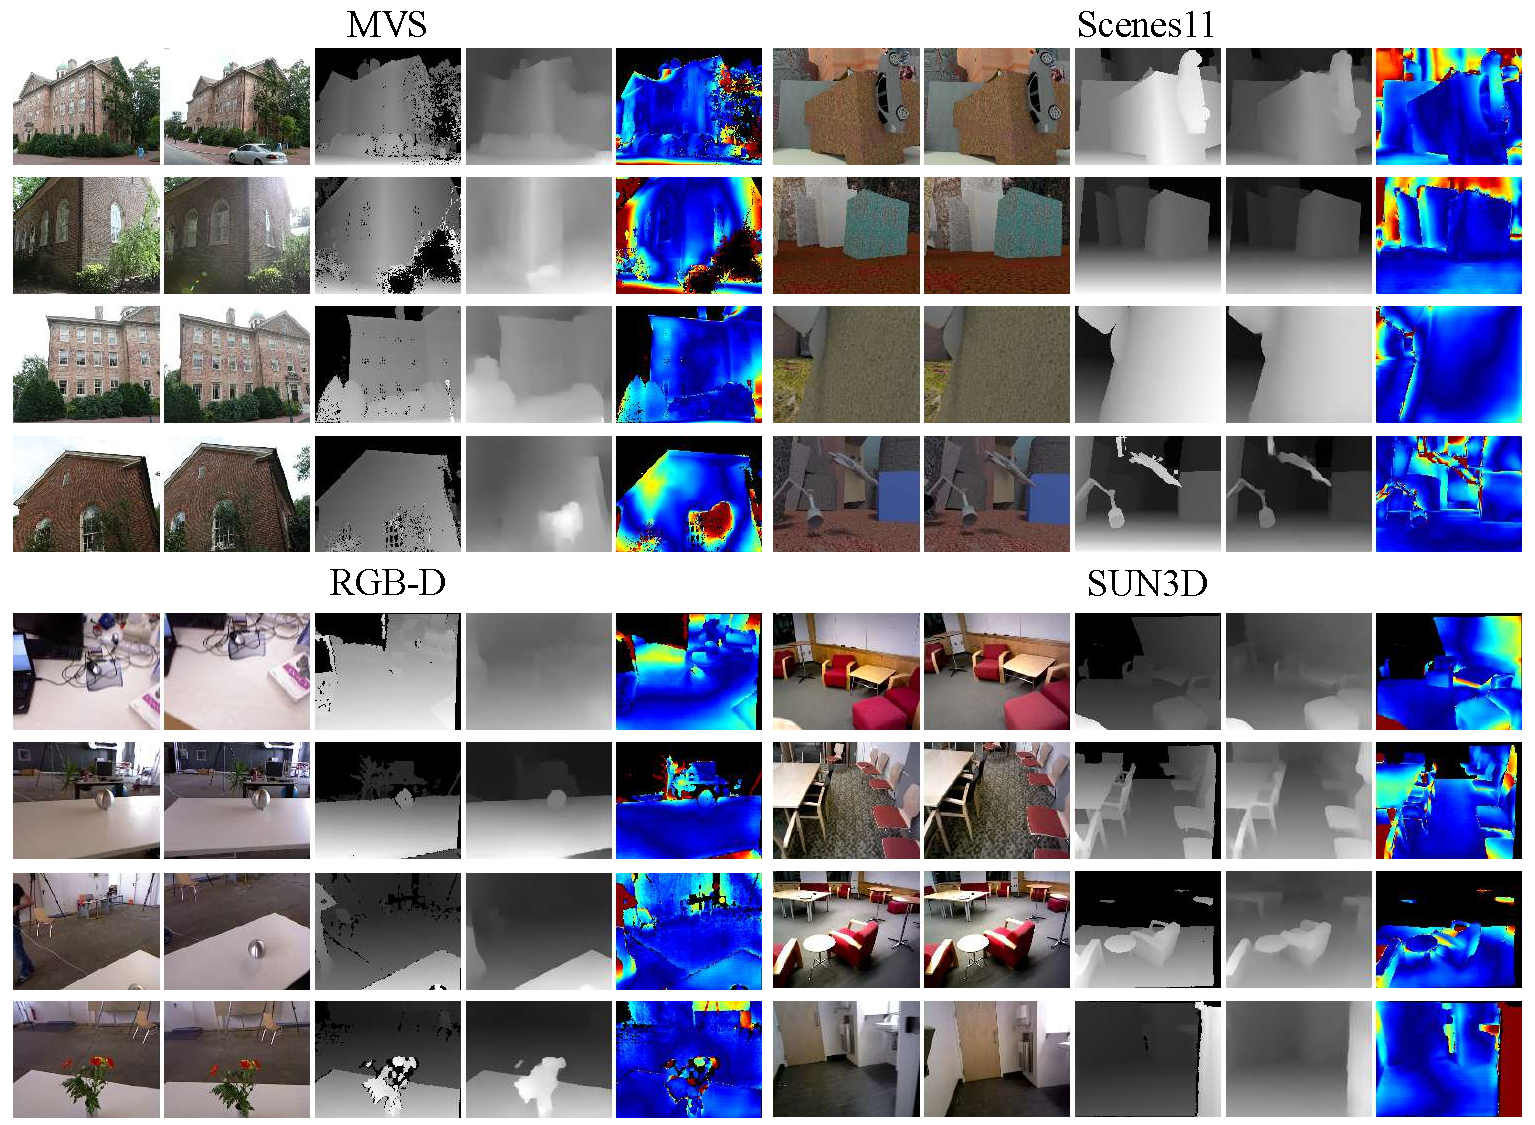
\includegraphics[width=1.0\linewidth]{figs/sup_demon.pdf}
\end{center}
    % \vspace{-0.5cm}
\caption{Depth map estimation of the DeMoN dataset. For each sample, from left to right: source image, target image, ground truth depth map, estimated depth map, and the L1-rel error map.}
   
\label{fig:sup_demon}
\end{figure*}
\begin{figure*}[h]
\begin{center}
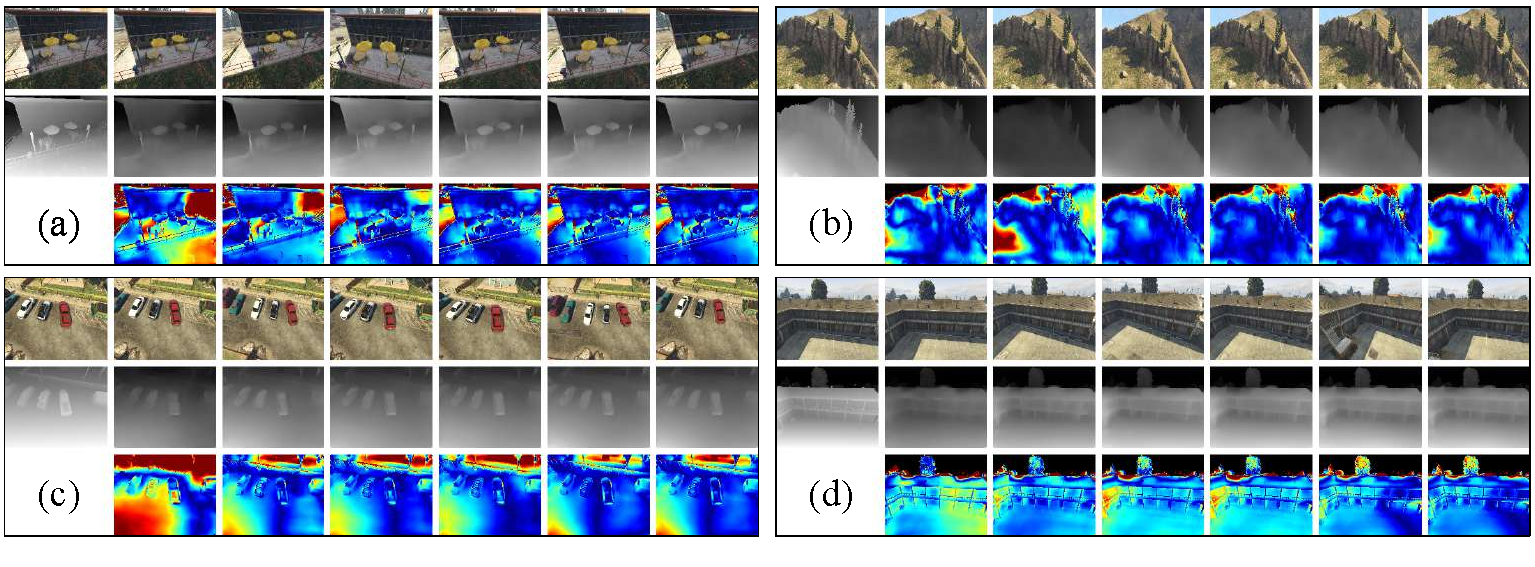
\includegraphics[width=1.0\linewidth]{figs/gta_multiview2.pdf}
\end{center}
\vspace{-0.5cm}
\caption{Depth map quality given different numbers of target images. For each sample, the up row shows the source image $I_s$, and five target images (from $I_{t,1}$ to $I_{t,5}$). The middle row shows the ground truth depth map and estimated depth maps with different target images. The bottom row shows the L1-rel error maps of the estimation. For example, from left to right, the fourth column shows target image $I_{t,3}$, estimated depth map which uses $I_s$, $I_{t,1}$, $I_{t,2}$, and $I_{t,3}$ as input, and the corresponding error map.}
\label{fig:gta_multiview}
\end{figure*}

\begin{figure*}[h]
\begin{center}
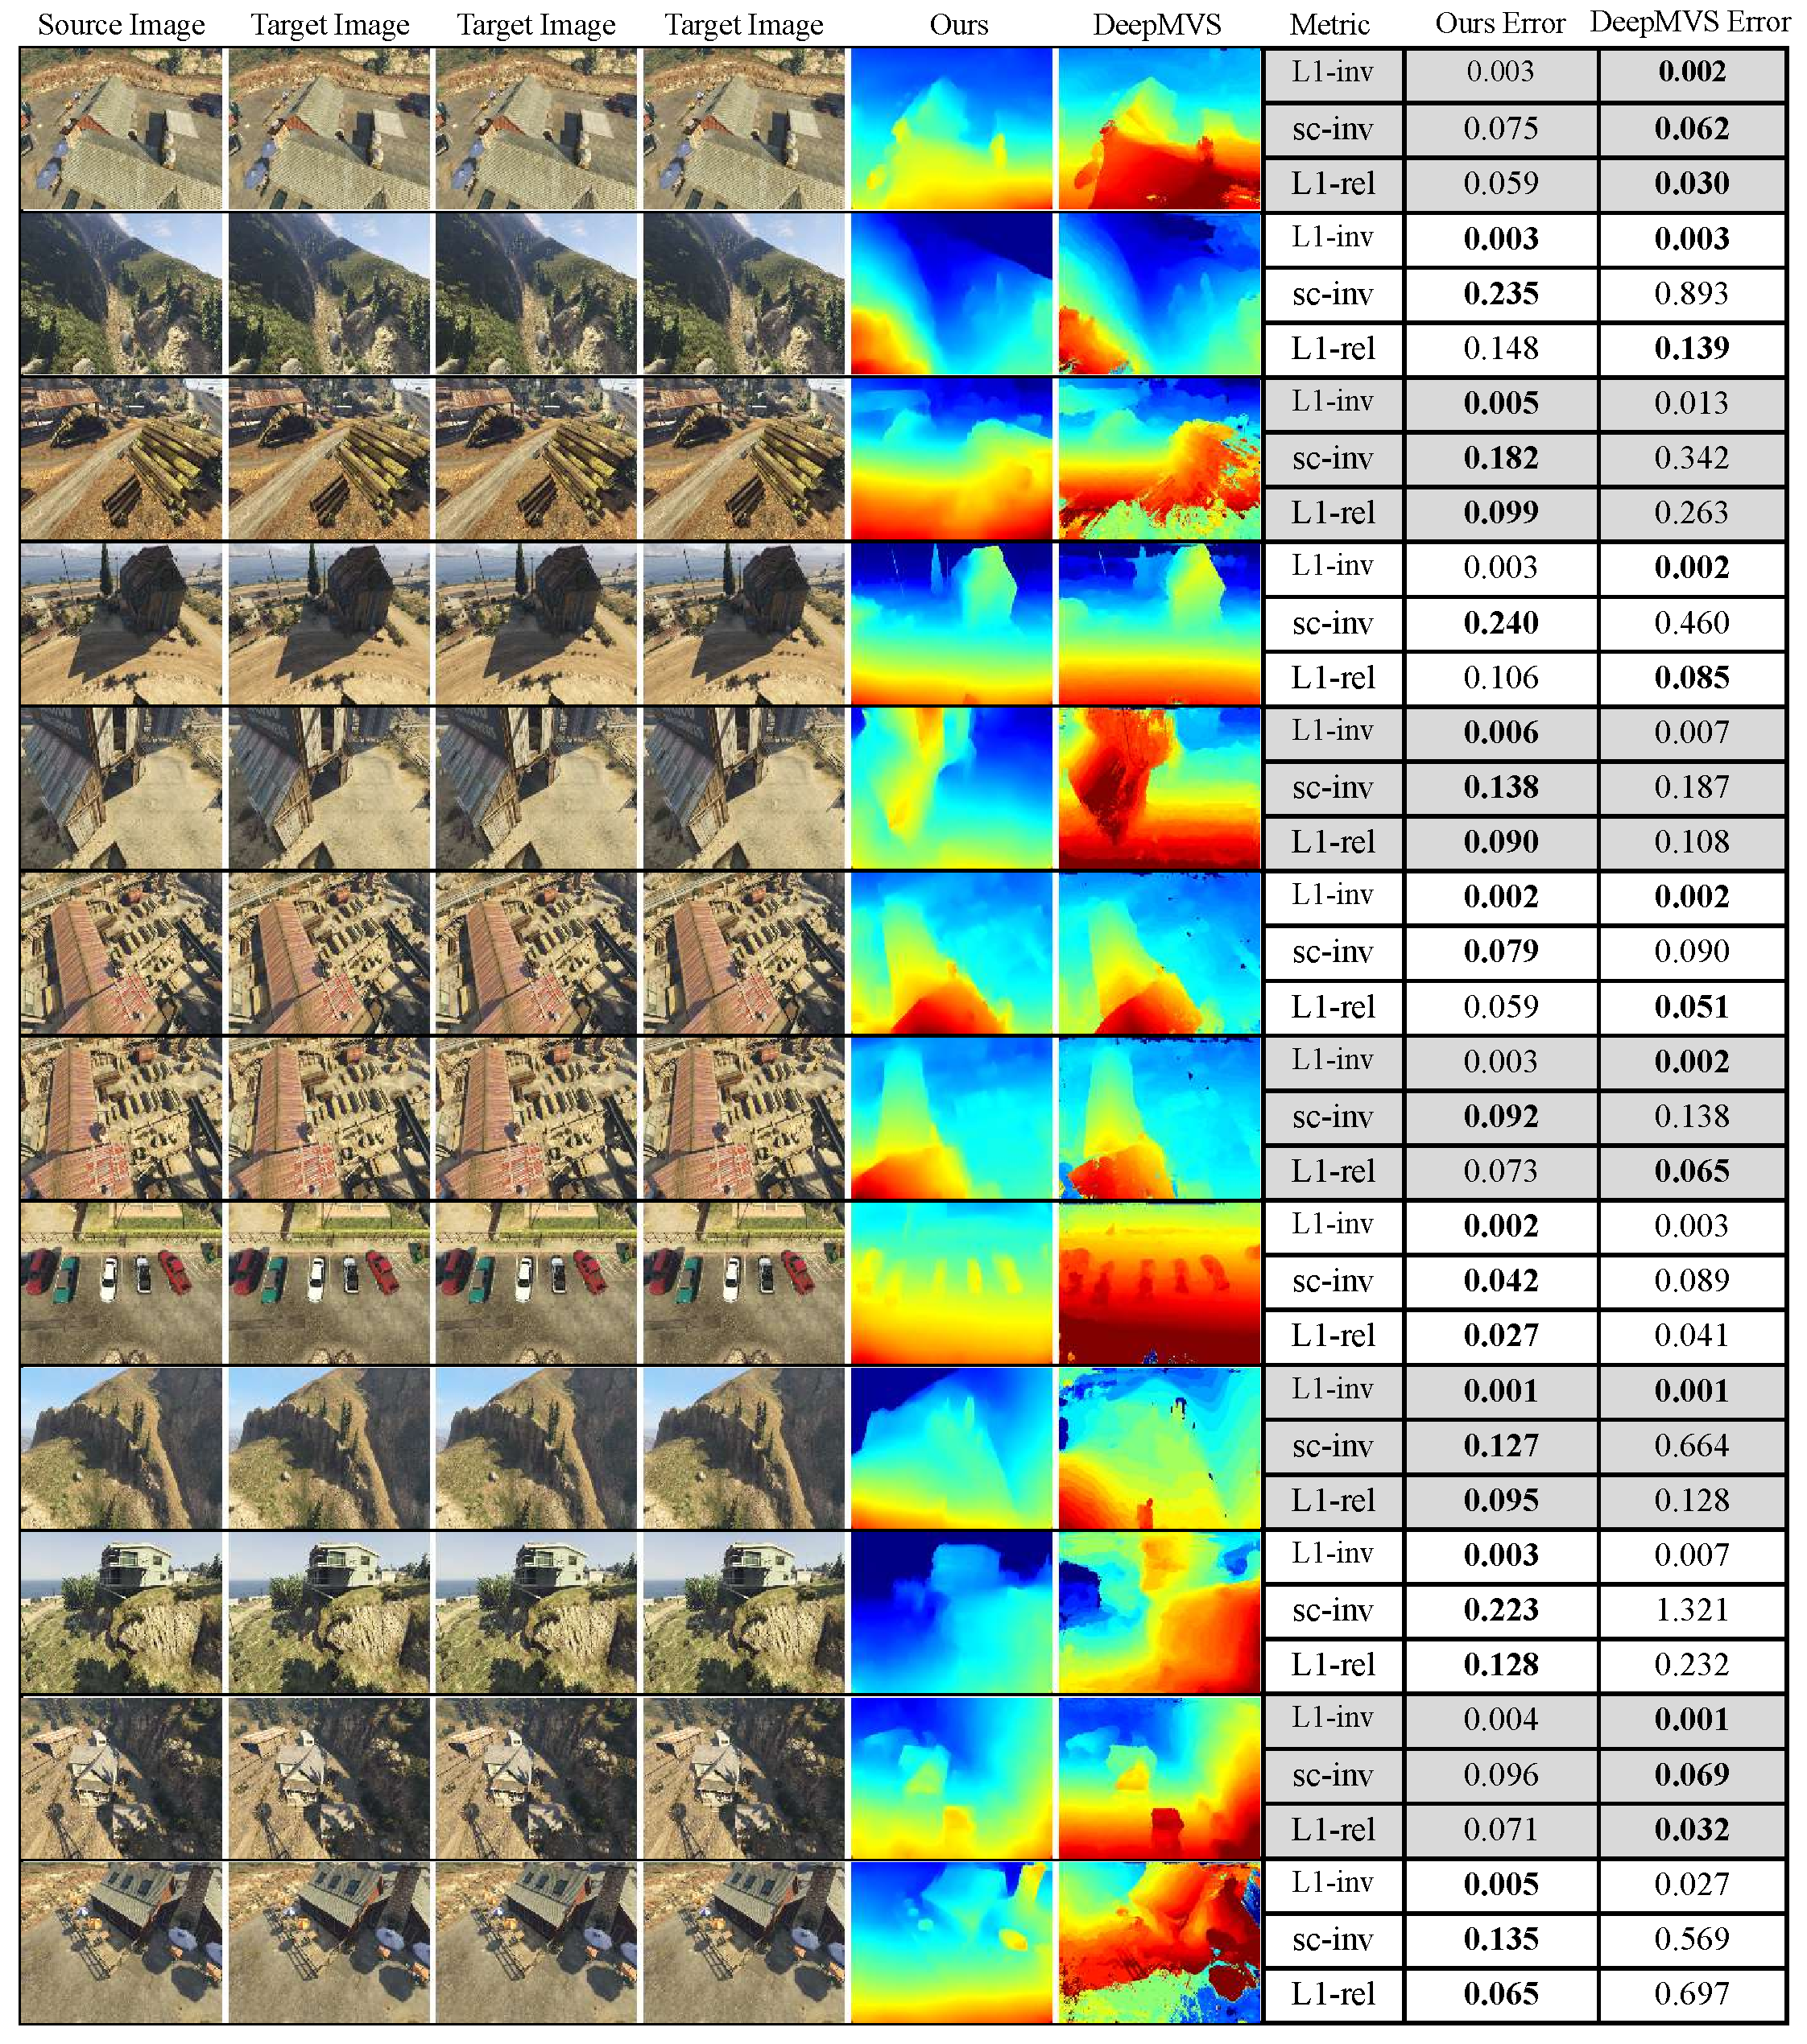
\includegraphics[width=1.0\linewidth]{figs/compare_mvs.pdf}
\end{center}   
\vspace{-0.5cm}
\caption{Depth comparison between our method and DeepMVS using \textit{randomly} sampled images. The right side is the calculated depth error. Best results are highlighted in bold. As shown, our method estimates smooth and detailed depth maps, and is much more efficient than DeepMVS.}
\label{fig:compare_mvs}
\end{figure*}
 
\begin{figure*}[h]
    % \vspace{-2.0cm}
\begin{center}
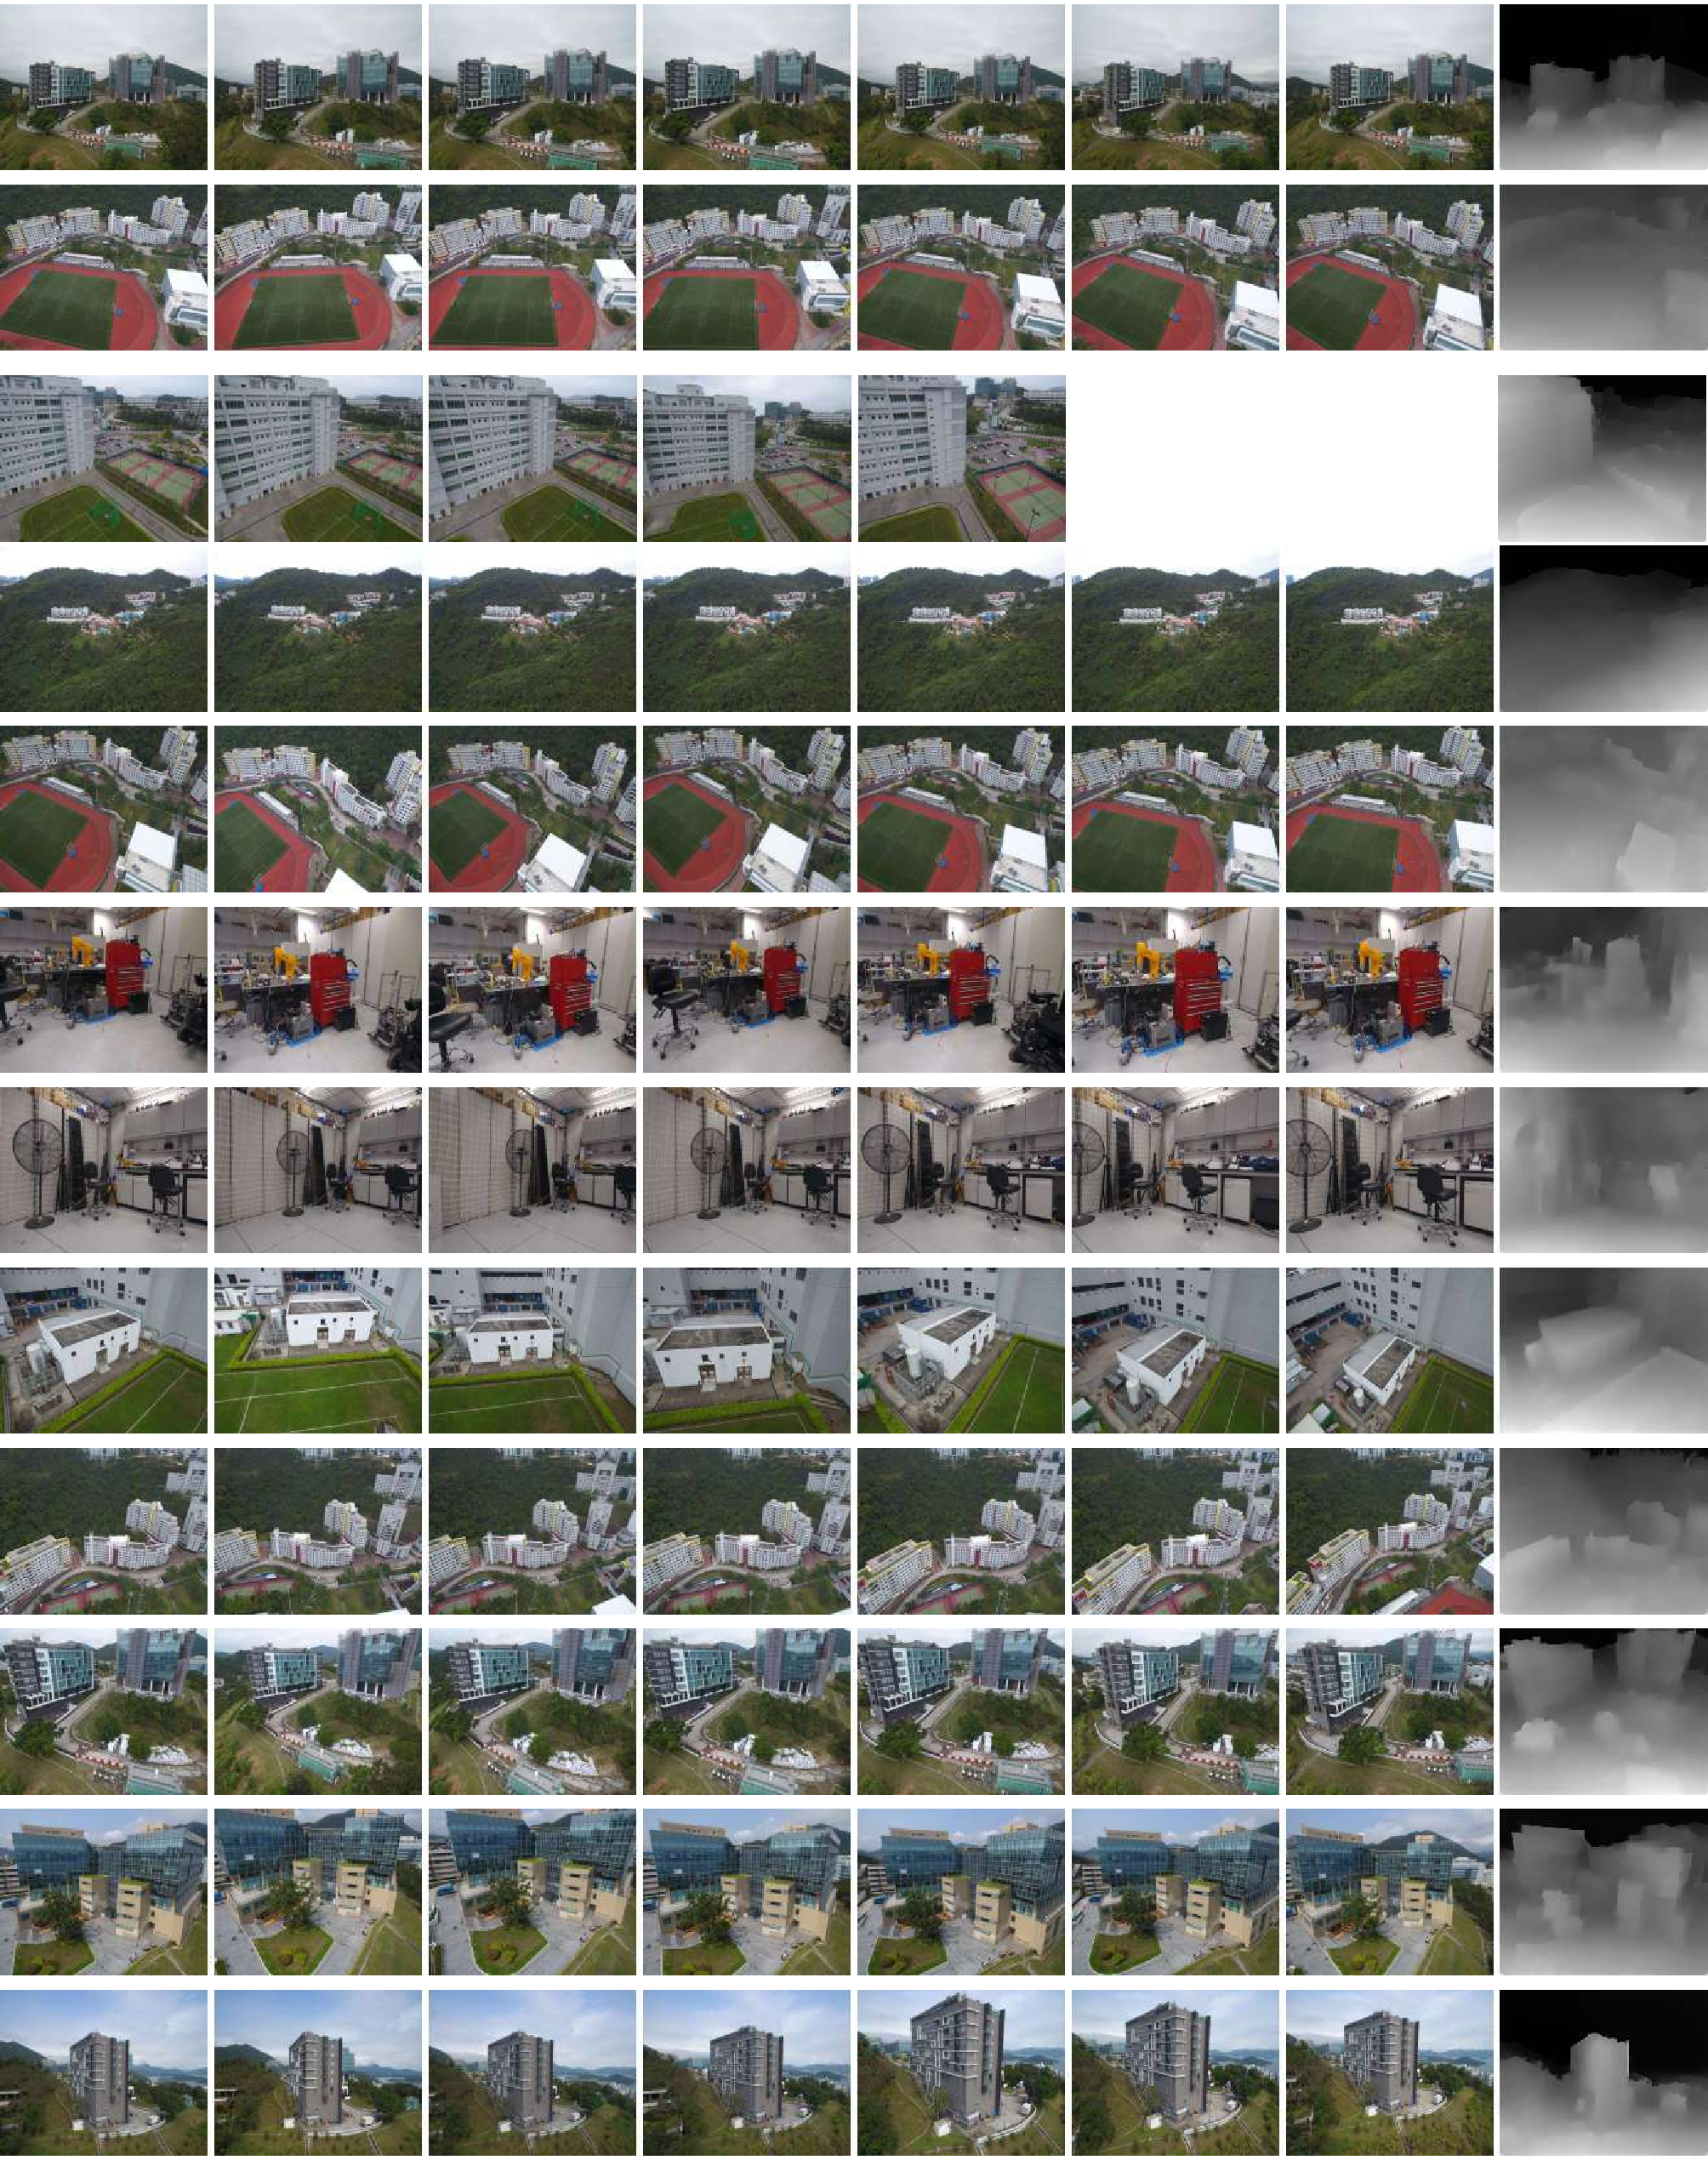
\includegraphics[width=0.9\linewidth]{figs/dji.pdf}
\end{center}
\caption{Applying the GTA-SfM trained models to aerial photographs and indoor images. From left to right in each row is the source image, target images, and the estimated depth map. The source image on the third row is observed by four target images, and other source images are observed by six target images.}
\label{fig:dji}
    % \vspace{-0.5cm}
\end{figure*}
 
\begin{figure*}[h]
    % \vspace{-2.0cm}
\begin{center}
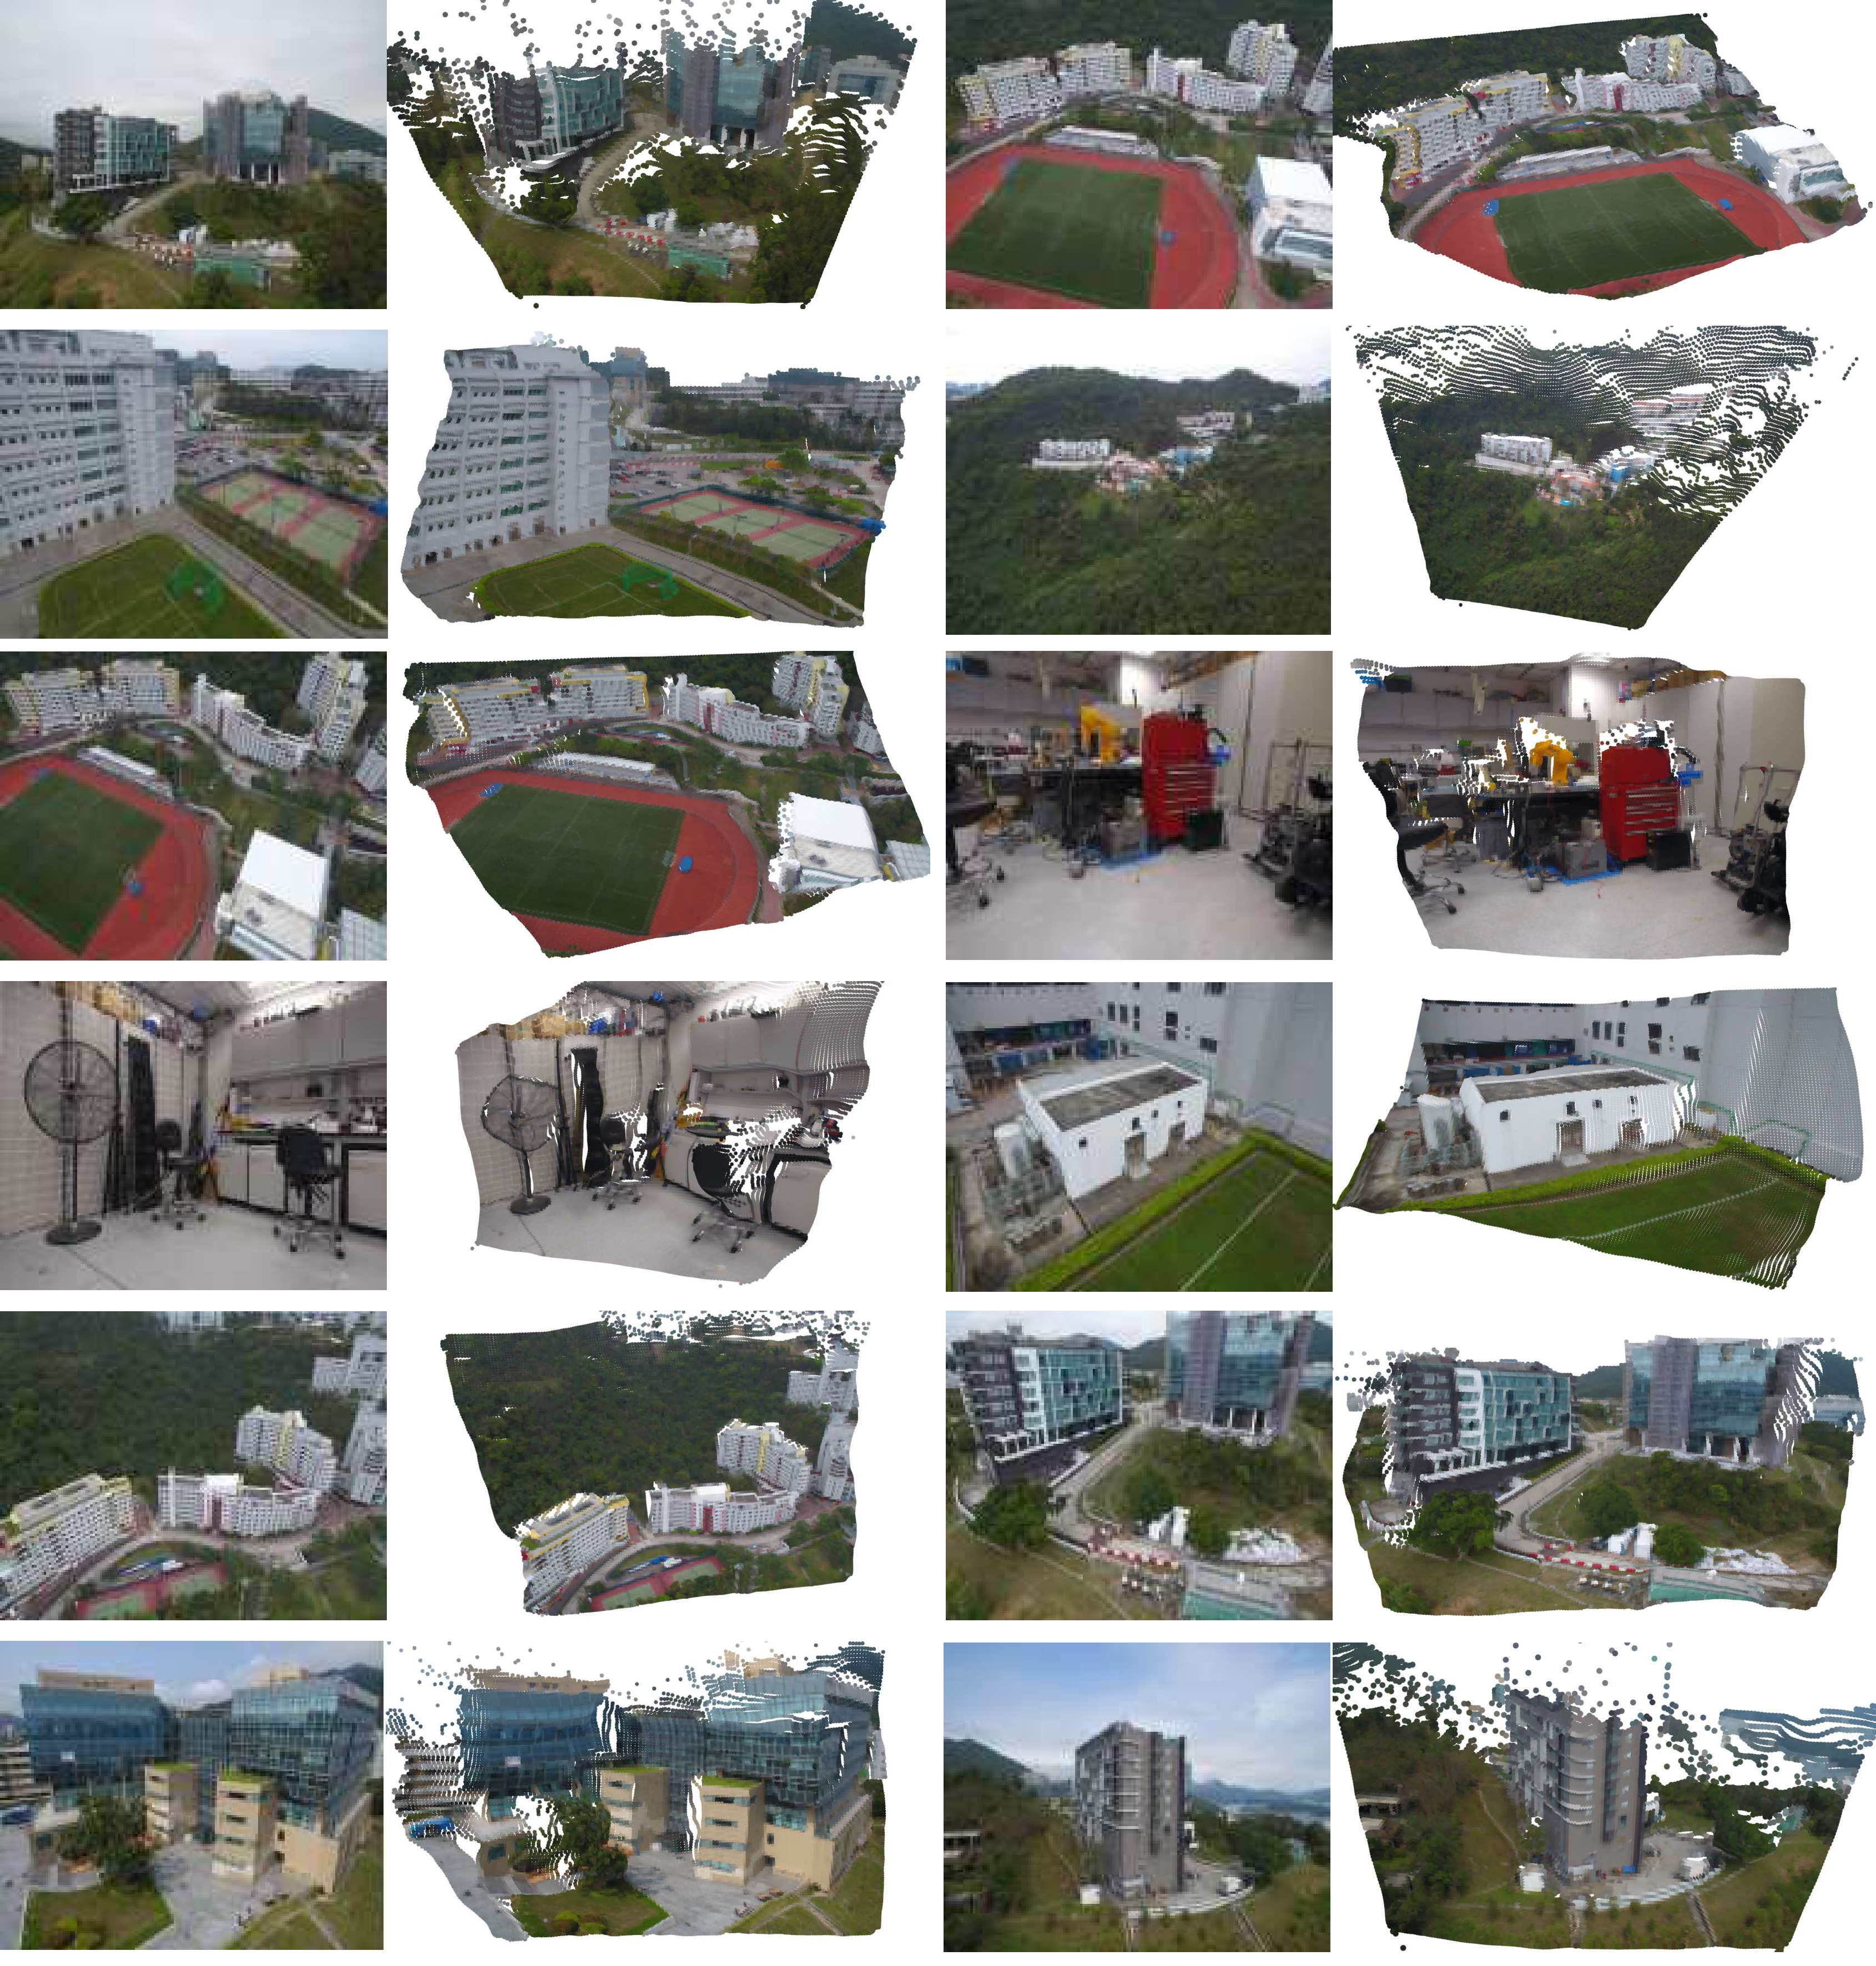
\includegraphics[width=1.0\linewidth]{figs/dji2.pdf}
\end{center}
\caption{Corresponding point cloud visualization of the estimated depth maps in Figure~\ref{fig:dji}. In each sample, left is the source image and right is the rendered point cloud. Pixels with depth larger than $200$ are considered as the sky and not visualized.}
\label{fig:dji2}
    % \vspace{-0.5cm}
\end{figure*}
 
\begin{figure*}[h]
    % \vspace{-2.0cm}
\begin{center}
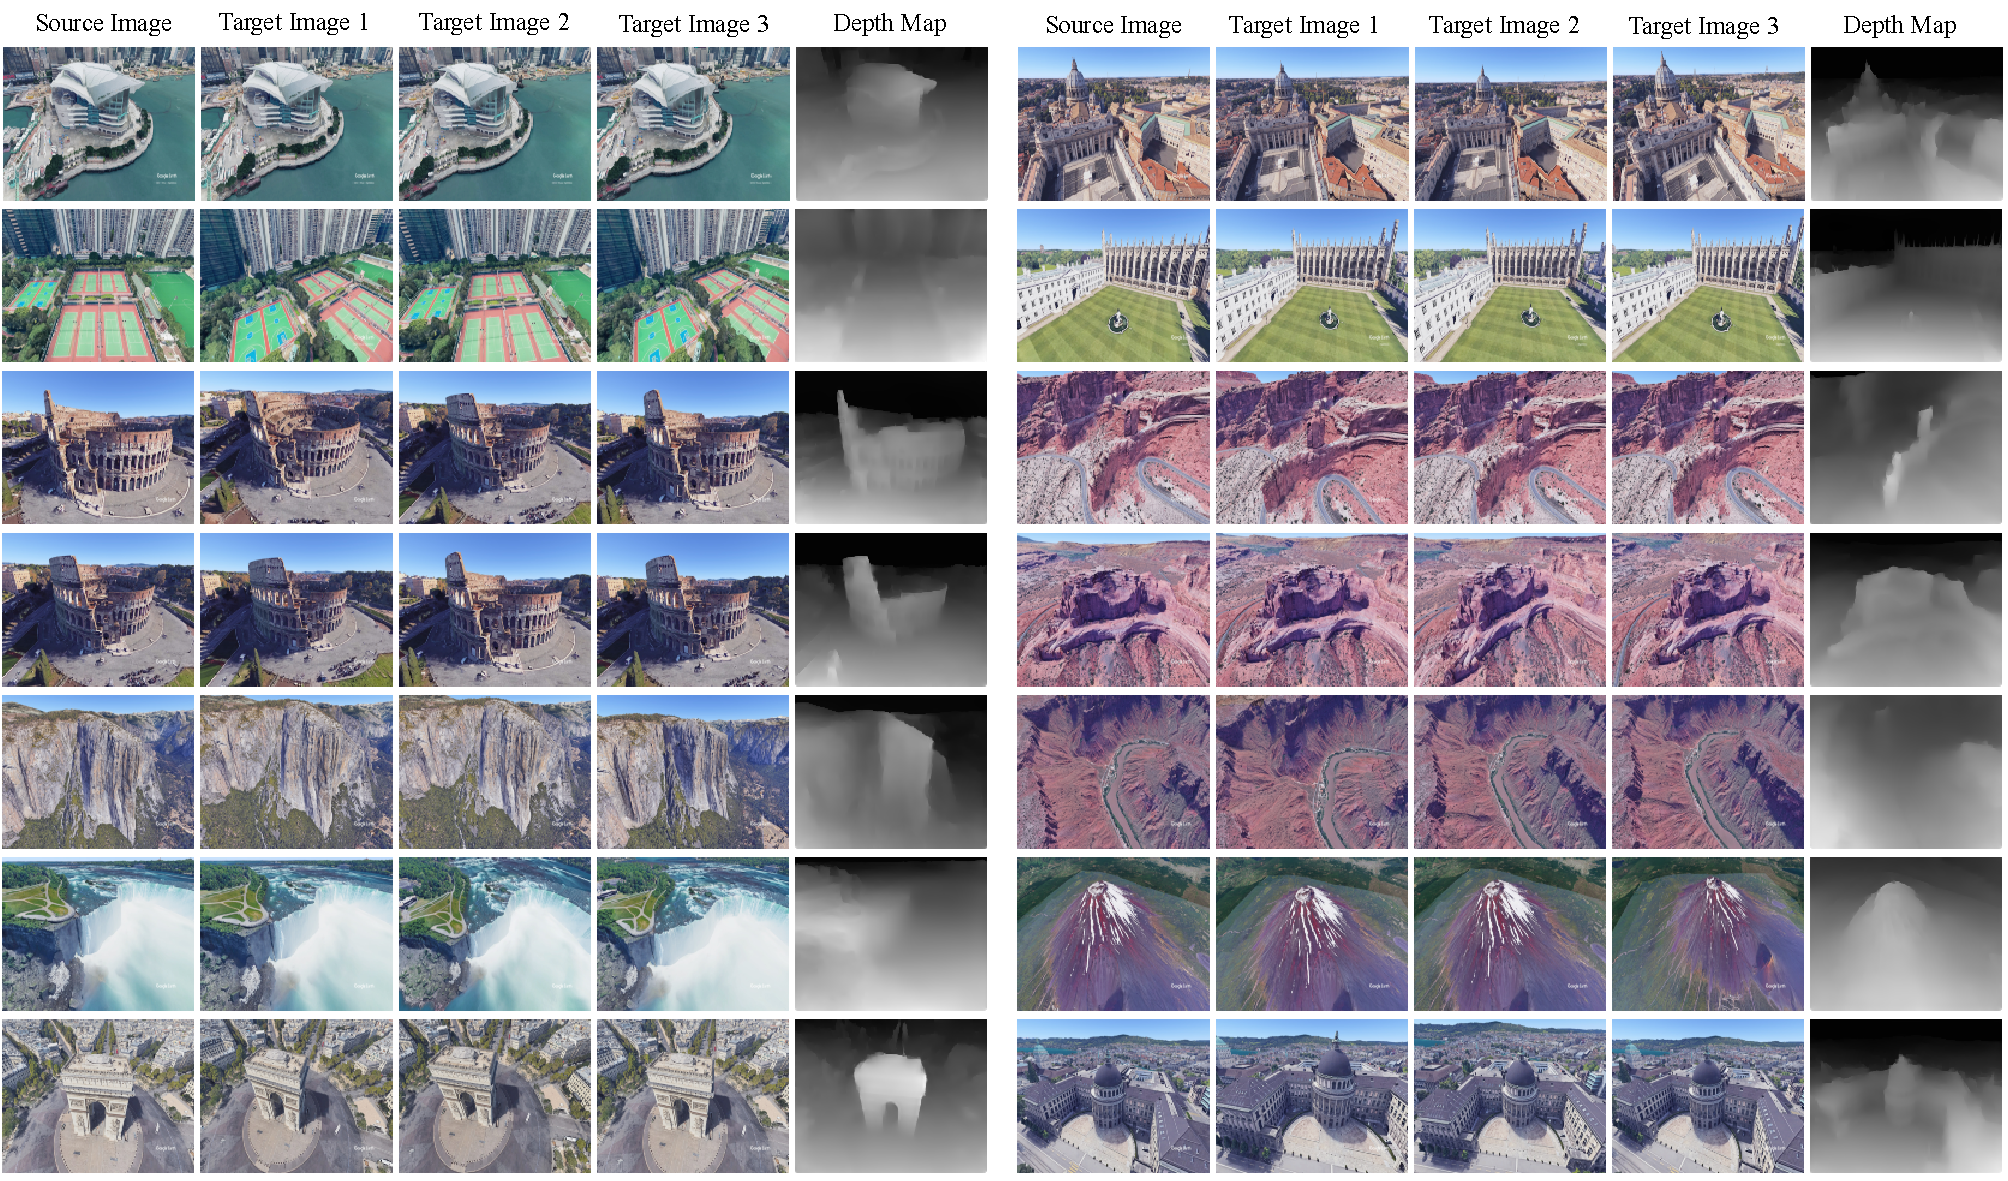
\includegraphics[width=1.0\linewidth]{figs/google_earth_re.pdf}
\end{center}
\caption{Applying the GTA-SfM trained models to reconstruct images from Google Earth. Different scenes are used to show the generalization ability of the proposed method.} 
\label{fig:google_earth}
    % \vspace{-0.5cm}
\end{figure*}
 
\begin{figure*}[h]
    % \vspace{-2.0cm}
\begin{center}
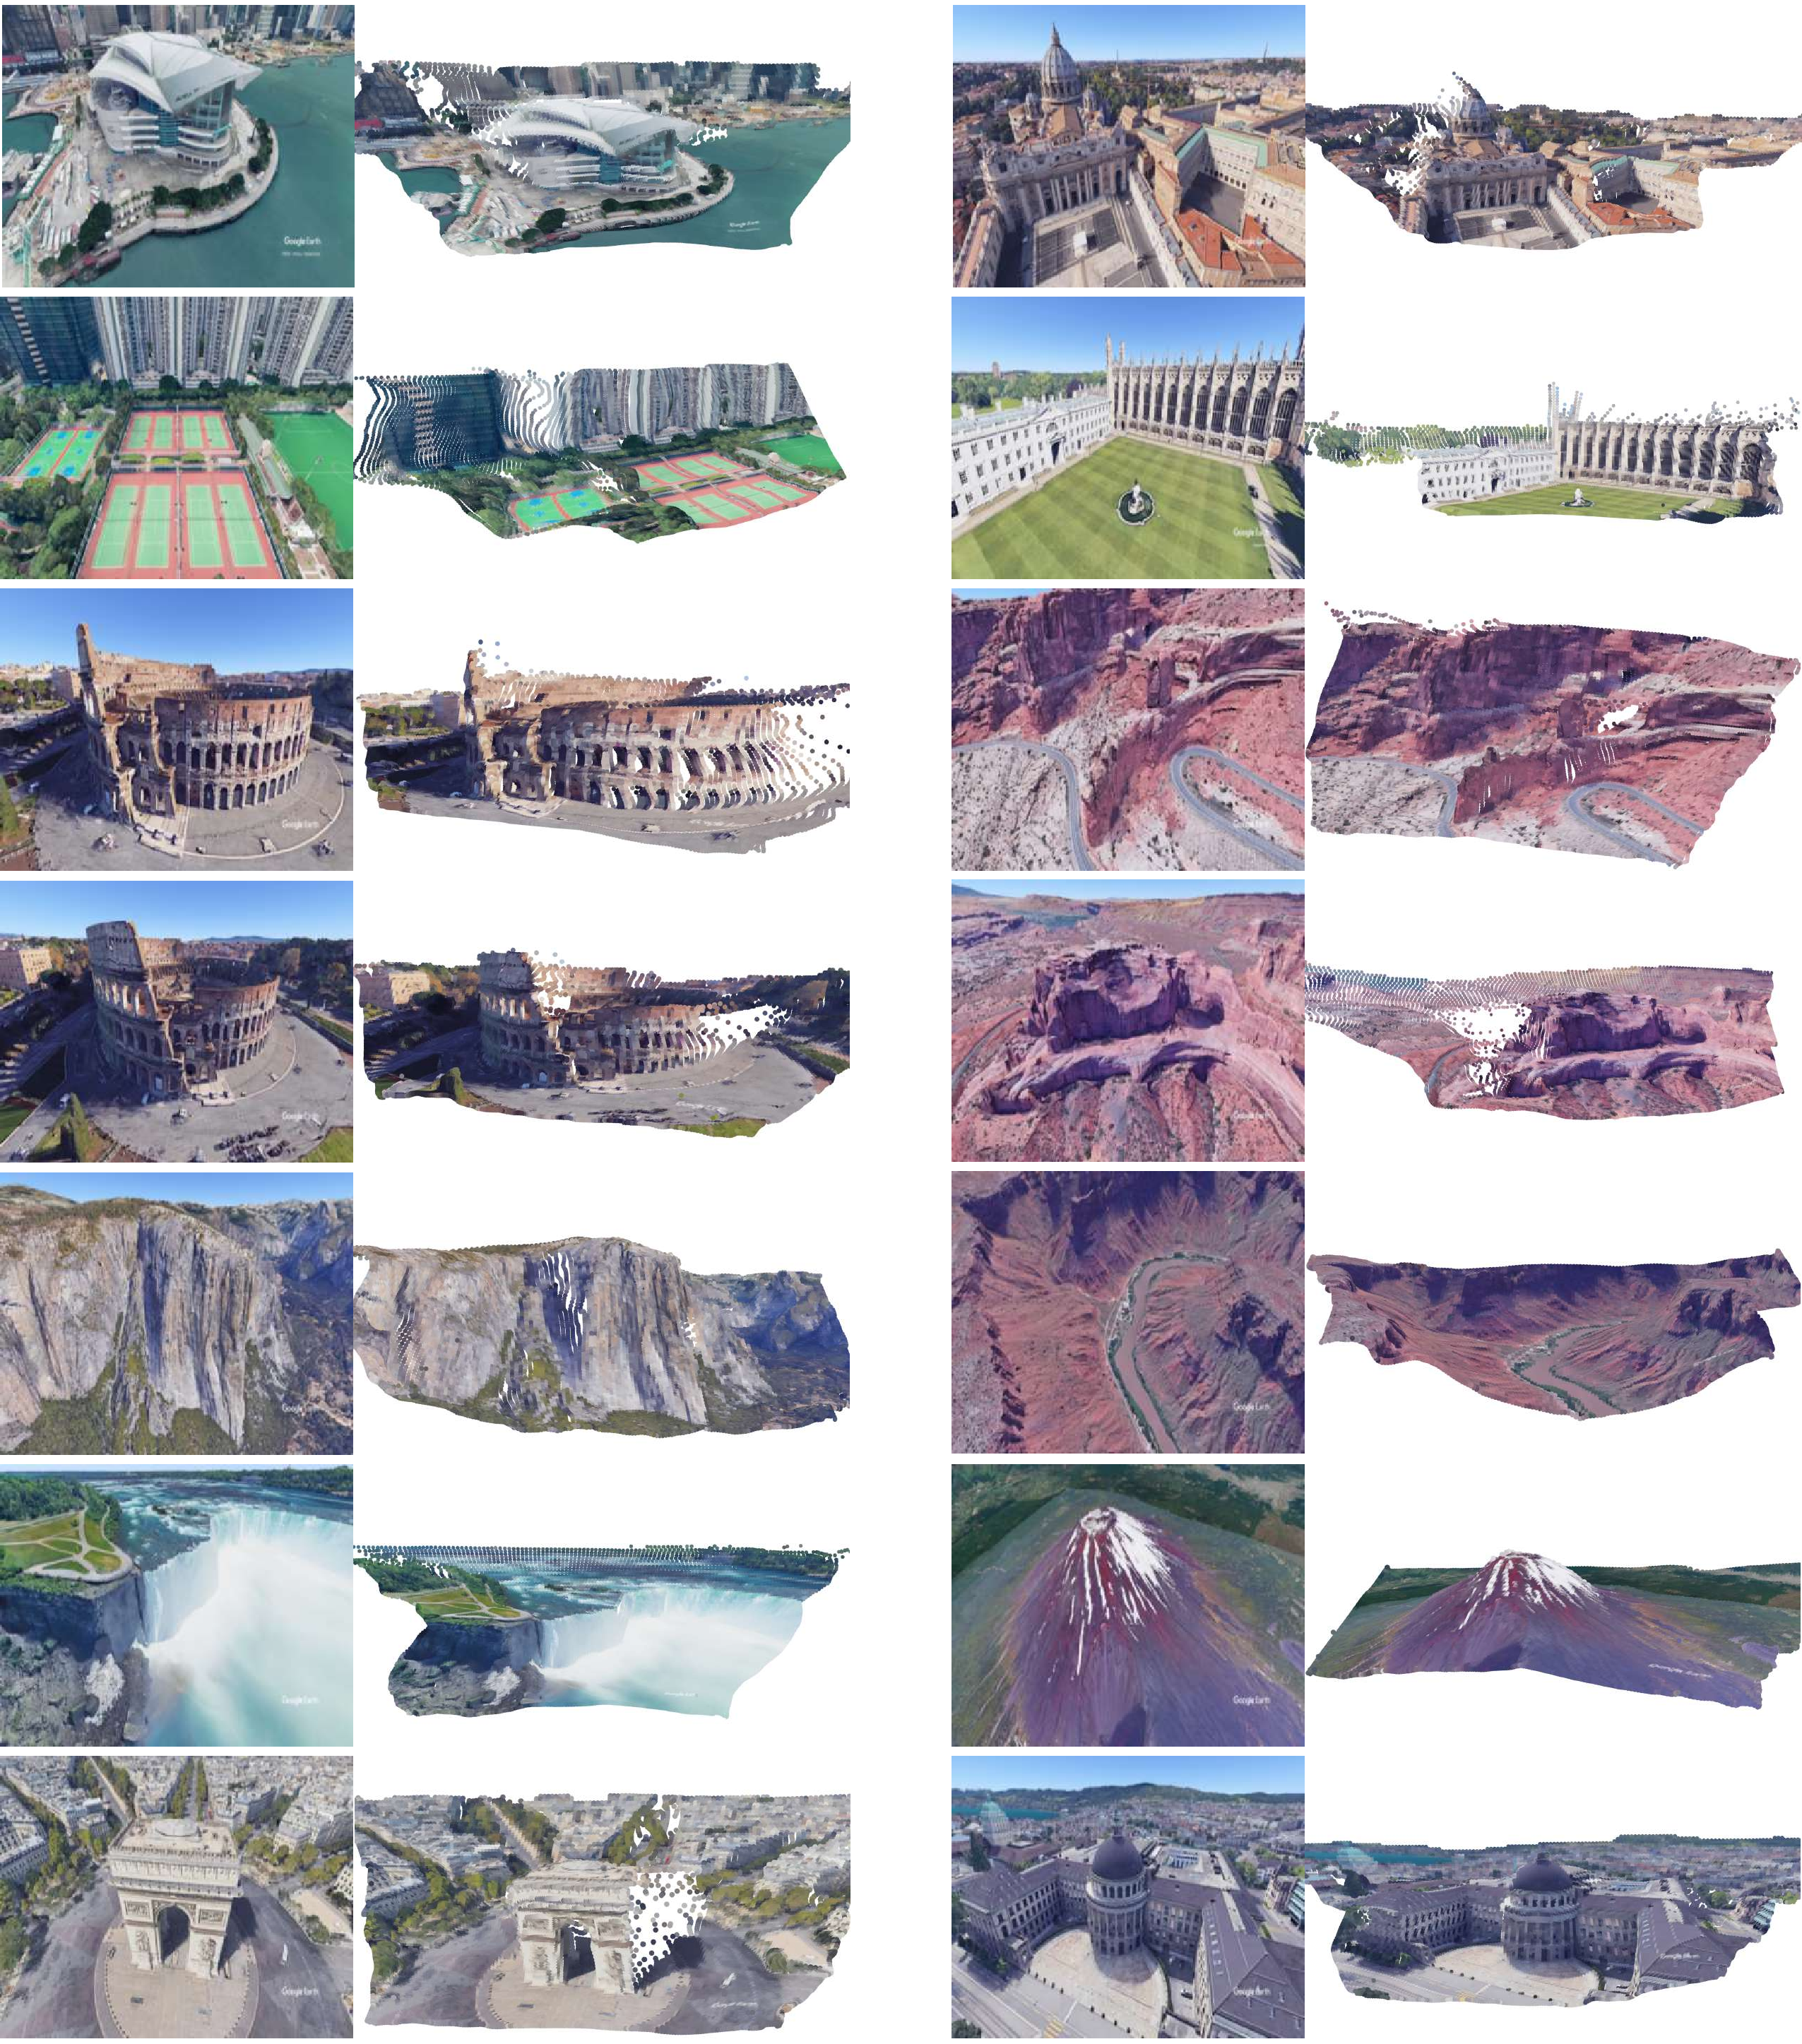
\includegraphics[width=0.9\linewidth]{figs/google_earth_re_pointcloud.pdf}
\end{center}
    % \vspace{-0.2cm}
    \caption{Point cloud visualization of reconstructed images from Google Earth.}
\label{fig:pointcloud}
    % \vspace{-0.5cm}
\end{figure*}
 
\begin{figure*}[h]
    % \vspace{-2.0cm}
\centering
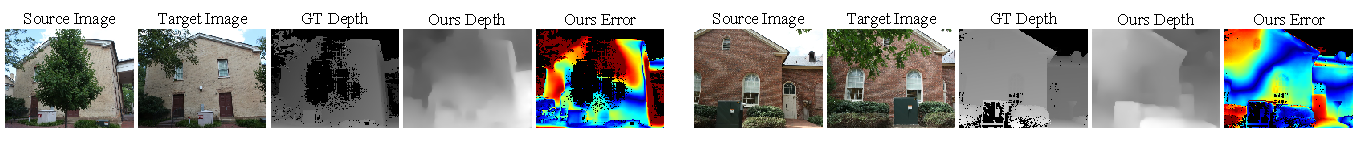
\includegraphics[width=1.0\linewidth]{figs/occlusion.pdf}
    % \vspace{-0.5cm}
\caption{Occlusion problem in the MVS sequence. Our method utilizes the multiview observations to triangulate the depth of each pixel thus the depth of occluded parts is difficult to be estimated. Even `ground truth' method cannot deal with such occlusion problems.}
\label{fig:occlusion}
    % \vspace{-0.5cm}
\end{figure*}
 
\end{document}
